\documentclass[11pt, a4paper, twoside]{report}
\usepackage[utf8x]{inputenc}
\usepackage[spanish]{babel}
\usepackage{lmodern}
\usepackage[T1]{fontenc}
\usepackage[top=2.5cm, bottom=2.25cm, outer=2.75cm, inner=2.75cm, heightrounded, marginparwidth=2.5cm, marginparsep=0.3cm]{geometry}	%márgenes
\usepackage{tabu}
\usepackage{pdfpages}
\usepackage{fancyhdr}

% Indicador completo en lugar de página
\fancyfoot[C]{{\ttfamily RTF PKT:CU \quad \thepage}}
\renewcommand*{\headrulewidth}{0pt}
\pagestyle{fancy}

\newcommand*{\PKT}{P\lower2pt\hbox{K}\kern-2pt\raise2pt\hbox{T}\kern-2pt}

\begin{document}

	% Título
	\begin{center}
		\scshape \large Acta de la Revisión Técnica Formal \textit{Casos de uso} - \PKT\ \vspace{.5cm}
	\end{center}

	En Madrid, a 8 de marzo de 2013 a la 13:02, reunidos de una parte Jaime Dan Porras y Alejandro Villarín Prieto,
representantes de \PKT\ y de otra Rubén Rafael Rubio Cuéllar y Sandra Bermejo	% ¿Sandra? Fue Juanan 
en representación de \textsc{Grupo Diedral}, se procede a la puesta en común de la revisión técnica formal de \textsc{Documento de casos de uso} de \PKT\ que \textsc{Grupo Diedral} ha realizado. \\

Se presenta a la reunión por parte de \textsc{Grupo Diedral} el documento objeto de revisión con los apartados a comentar durante la reunión (se adjunta a este acta). \\


A continuación se exponen las conclusiones a las que se llega durante la reunión, 

	\begin{quotation} \itshape
			Las sugerencias y errores que presenta \textsc{Grupo Diedral} son plenamente\break aceptados y
			se tendrán en consideración para futuras revisiones del documento de casos de uso.

			\medskip
			En general, el documento de casos de uso no se ajusta en algunos casos a los estándares. Se encuentran términos de muy bajo nivel.
			Quedan sin explicar las razones de alguna secuencia alternativa, y por último el comienzo y final de los casos de uso es demasiado drástico.

			\medskip
			Se recomienda un examen del documento para solucionar estos problemas.
	\end{quotation}

	Por tanto, se el documento se declara \textsc{rechazado}.\\
	Ambas partes expresan la conformidad con lo hablado en la reunión.

\vspace{2cm}
\raggedleft{En Madrid, a 8 de marzo de 2013}

\raggedright
Los asistentes,

\vspace{2.5cm}

	\begin{tabu} to \linewidth {X[1,c] X[1, c]}
		Jaime Dan Porras & Alejandro Villarín Prieto
	\end{tabu}

	\vfill

	\begin{tabu} to \linewidth {X[1,c] X[1, c]}
		Rubén Rafael Rubio Cuéllar & Sandra Bermejo
	\end{tabu}
	
	\vfill

	{\itshape A continuación se incluye el anexo: }

	% Incluye el anexo del otro grupo
	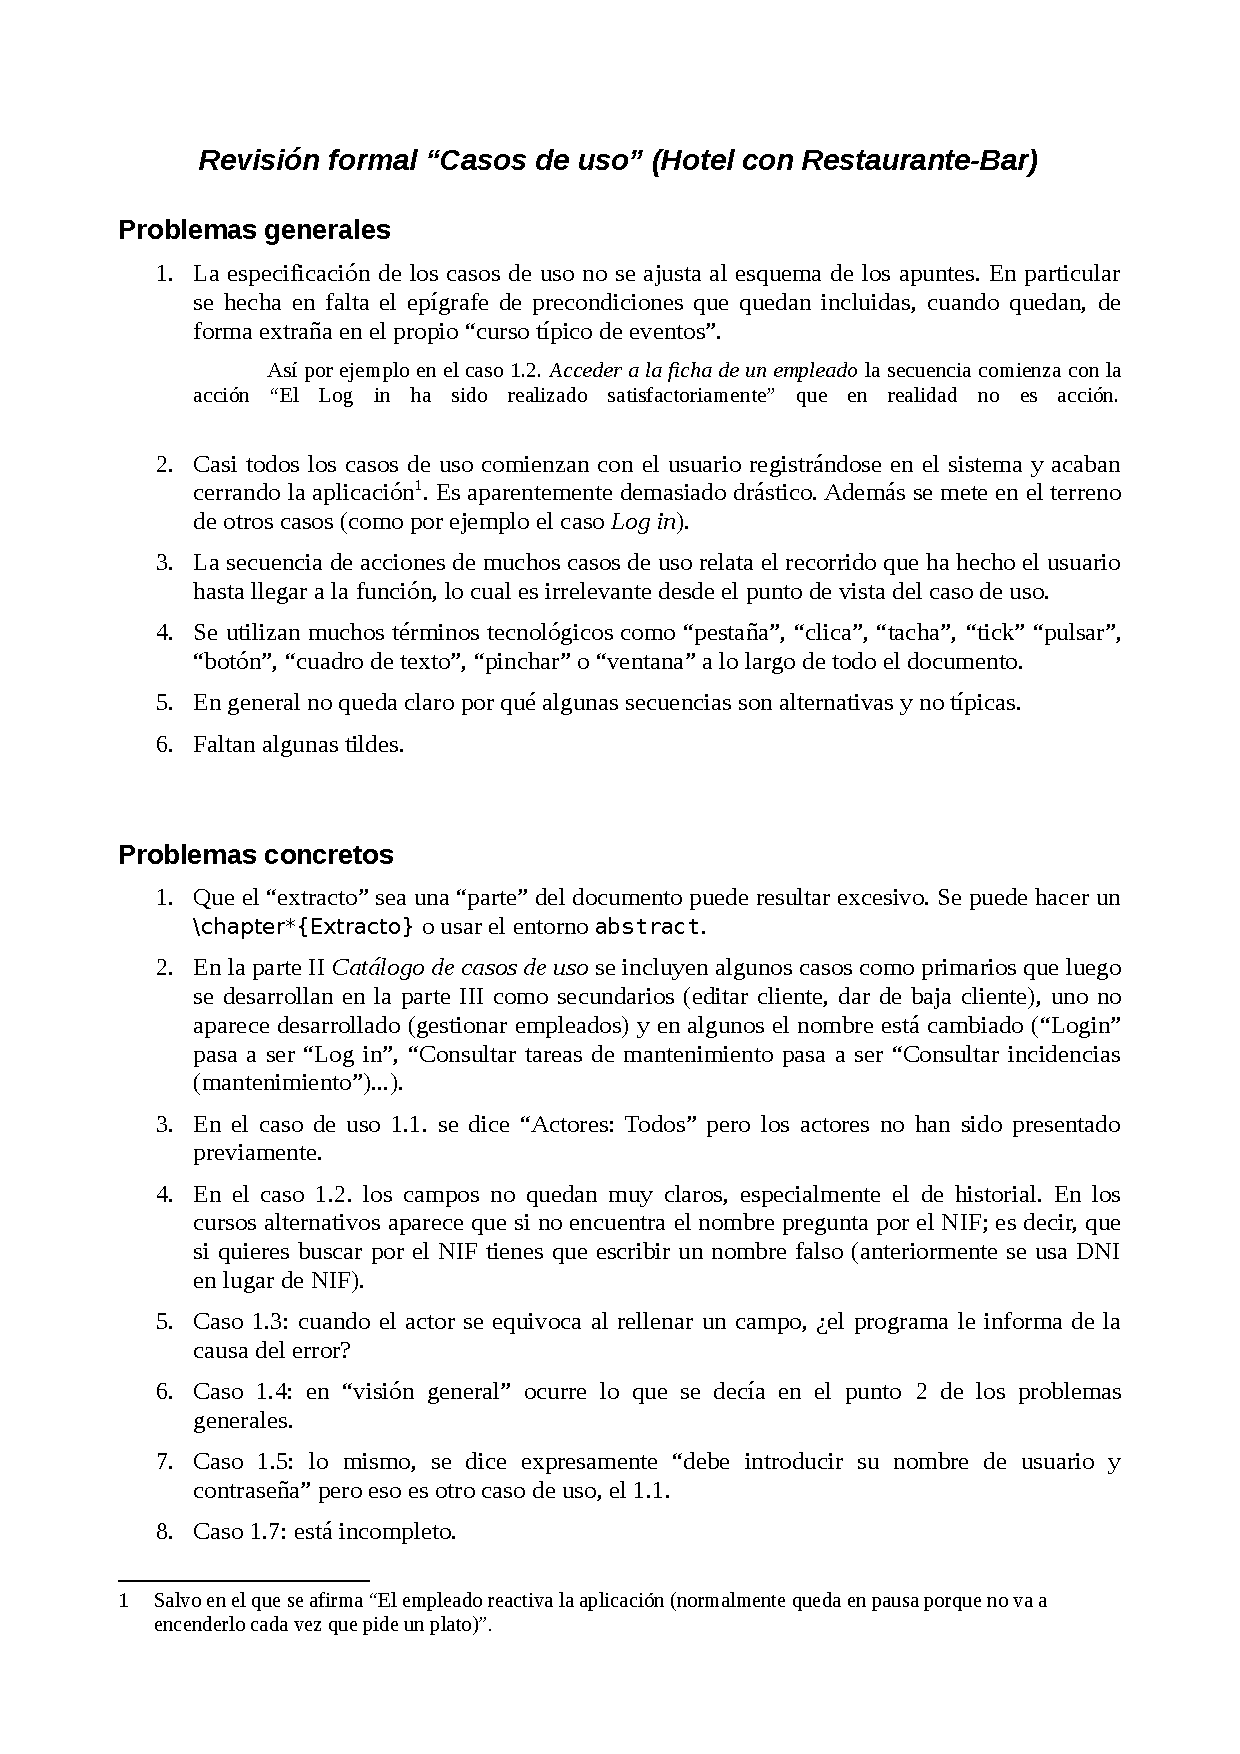
\includepdf[pages=1-2, pagecommand={}]{casosdeuso_pkt_anexo.pdf}
\end{document}
